\documentclass[aspectratio=169]{beamer}
\useoutertheme[progressbar=frametitle]{metropolis}
\useinnertheme{metropolis}
\definecolor{nabgray}{rgb}{0.6,0.59,0.61}
\usecolortheme[named=nabgray]{structure}
\usepackage{tikz}
\usepackage[utf8]{inputenc}
\usepackage[spanish]{babel}
\usepackage{fontspec}
\setmonofont{JetBrains Mono}
\setmainfont{Roboto}
\setsansfont{Roboto}

\usepackage{smartdiagram}
\usepackage{qtree}
\usepackage{verbatim}
\usepackage{svg}
\usepackage{graphicx}
\usepackage{color}
\definecolor{lightgray}{rgb}{0.95, 0.95, 0.95}
\definecolor{darkgray}{rgb}{0.4, 0.4, 0.4}
\definecolor{ocherCode}{rgb}{1, 0.5, 0} % #FF7F00 -> rgb(239, 169, 0)
\definecolor{blueCode}{rgb}{0, 0, 0.93} % #0000EE -> rgb(0, 0, 238)
\definecolor{greenCode}{rgb}{0, 0.6, 0} % #009900 -> rgb(0, 153, 0)

\usepackage{upquote}
\usepackage{listings}
\lstset{language=java,
    otherkeywords={var,record},
	% Basic design
	backgroundcolor=\color{lightgray},
	basicstyle={\small\ttfamily},
	frame=l,
	keywordstyle=\footnotesize\color{blue},
	escapeinside={<@}{@>},
	breaklines=true,
	% Line numbers
	xleftmargin={0.75cm},
	numbers=left,
	stepnumber=1,
	firstnumber=1,
	numberfirstline=true
	% Code design
	identifierstyle=\color{black},
	keywordstyle=\color{ocherCode}\bfseries,
	ndkeywordstyle=\color{greenCode}\bfseries,
	stringstyle=\color{ocherCode}\ttfamily,
	commentstyle=\color{darkgray}\ttfamily,
	tabsize=2,
	showtabs=true,
	showspaces=false,
	showstringspaces=false,
	extendedchars=true,
	breaklines=true
}

\lstdefinelanguage{bash}{
    basicstyle=\ttfamily,
    showstringspaces=false,
    commentstyle=\color{red},
    keywordstyle=\color{blue},
    numbers=right,
    xleftmargin={0.25cm}
}

\usebackgroundtemplate
{
	
\includegraphics[width=\paperwidth]{Images/fondo}%
}


\title{Conceptos básicos de Kubernetes}
\author{Víctor Orozco - @tuxtor}
\institute{Academik}
\date{\today}

\begin{document}

{
    \usebackgroundtemplate{
\includegraphics[width=\paperwidth]{Images/portada}}
    \setbeamercolor{frametitle}{fg=red}
    \usebeamercolor[fg]{normal text}
    \frame{\titlepage}
}

\begin{frame}{El camino a Kubernetes}
    \begin{figure}
        \centering
        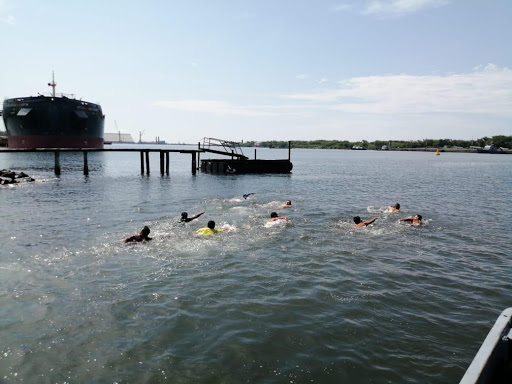
\includegraphics[width=0.5\linewidth]{Images/run}
    \end{figure}
\end{frame}


\begin{frame}{El camino a Kubernetes}
    \begin{figure}
        \centering
        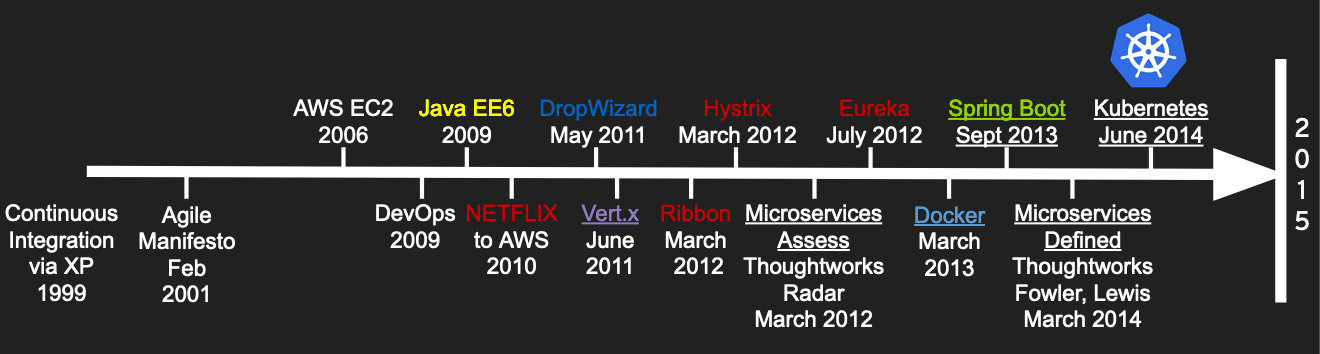
\includegraphics[width=\linewidth]{Images/timeline.png}
        \label{fig:container}
    \end{figure}

    Créditos: Rafael Benevides
\end{frame}

\begin{frame}{El camino a Kubernetes}
    \begin{figure}
        \centering
        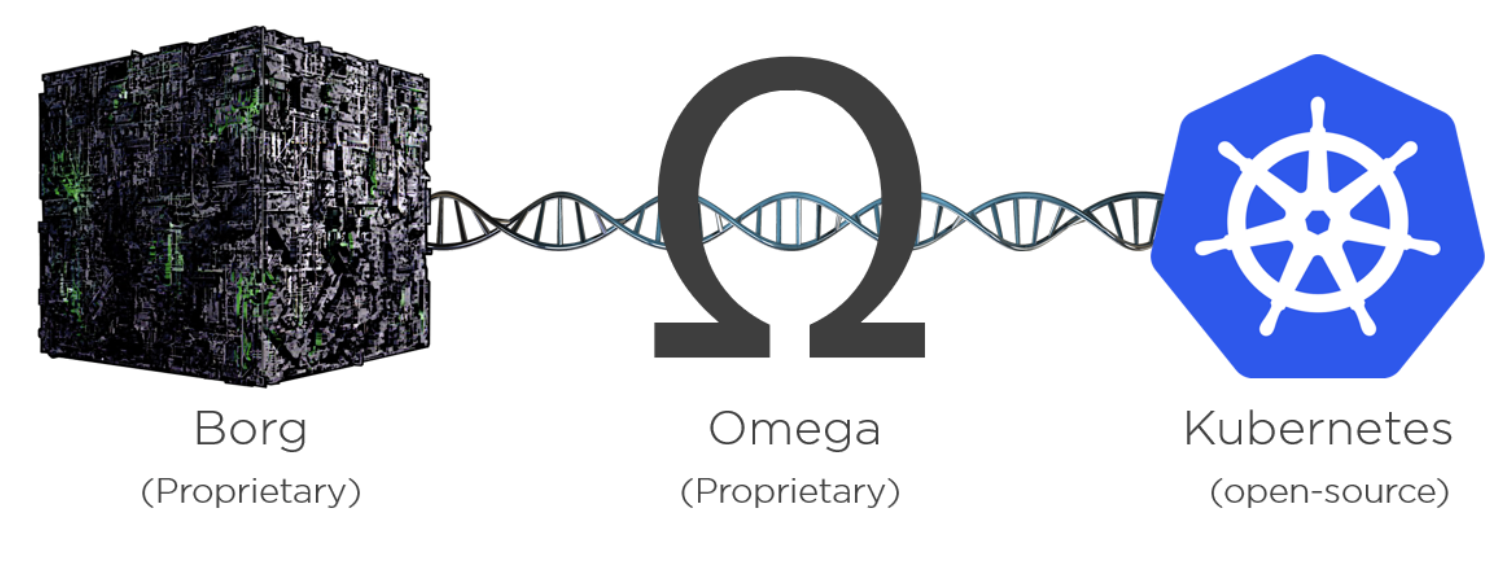
\includegraphics[width=\linewidth]{Images/borg.png}
    \end{figure}

\end{frame}




{
    \usebackgroundtemplate{
\includegraphics[width=\paperwidth]{Images/separador}}
    \setbeamercolor{normal text}{fg=white}
    \setbeamercolor{frametitle}{fg=red}
    \usebeamercolor[fg]{normal text}
    \section{Kubernetes desde 10k pies de altura}
}


\begin{frame}{Kubernetes}

    \begin{exampleblock}{Kubernetes}
Kubernetes \textbf{despliega y gestiona (orquesta)} aplicaciones que están empacadas para ser ejecutadas como contenedores y que están programadas de tal forma que escalan, son resilientes y pueden ser actualizadas, alineándose a los requerimientos de negocio modernos.
    \end{exampleblock}

\end{frame}

\begin{frame}{Kubernetes}

    \begin{alertblock}{¿Que es un Kubernetes?}
        \begin{itemize}
            \item Orquestador
            \item Gestiona aplicaciones y despliegues (en contenedores)
            \item Declarativo
            \item Elastico (scale up)
            \item Resiliente (self healing)
            \item Actualizaciones
        \end{itemize}
    \end{alertblock}

\end{frame}

\begin{frame}{Contenedores}

    \begin{exampleblock}{Contenedores}
        \begin{itemize}
            \item Docker
            \item Containerd
            \item Kata container
            \item CRI
            \item Runtime Classes
        \end{itemize}
    \end{exampleblock}

\end{frame}




\begin{frame}{Contenedores}
    \begin{figure}
        \centering
        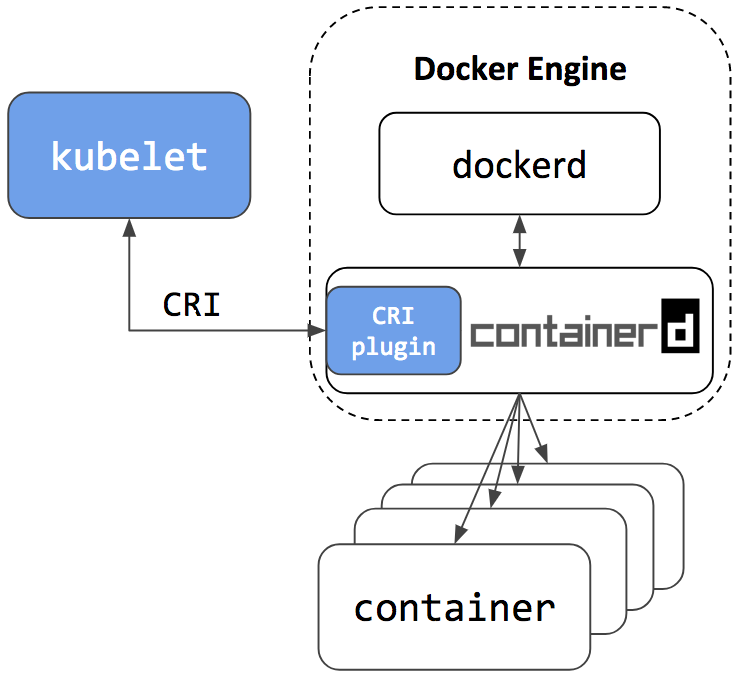
\includegraphics[width=0.4\linewidth]{Images/dockercontainerd.png}
    \end{figure}
Créditos: Nigel Poulton - The Kubernetes Book
\end{frame}

\begin{frame}{Contenedores}
    \begin{figure}
        \centering
        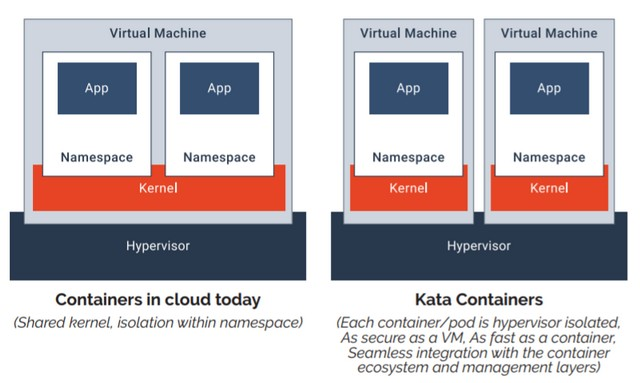
\includegraphics[width=0.5\linewidth]{Images/dockerkata.jpg}
    \end{figure}
\end{frame}

\begin{frame}{Kubernetes}
    \begin{figure}
        \centering
        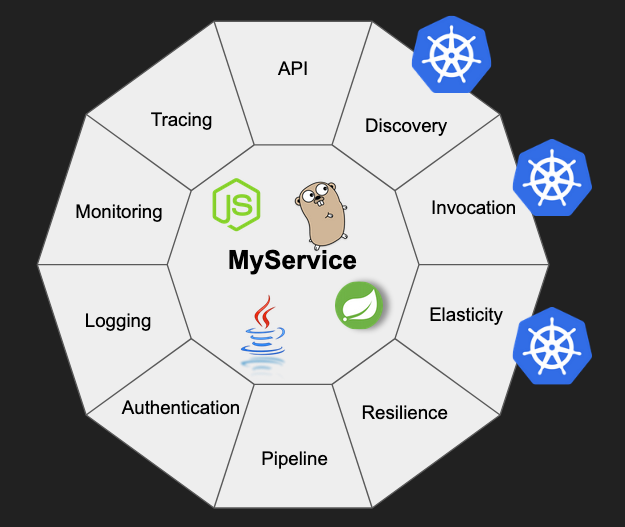
\includegraphics[width=0.5\linewidth]{Images/kube1.png}
        \label{fig:container}
    \end{figure}

    Créditos: Rafael Benevides
\end{frame}


\begin{frame}{Kubernetes}
    \begin{figure}
        \centering
        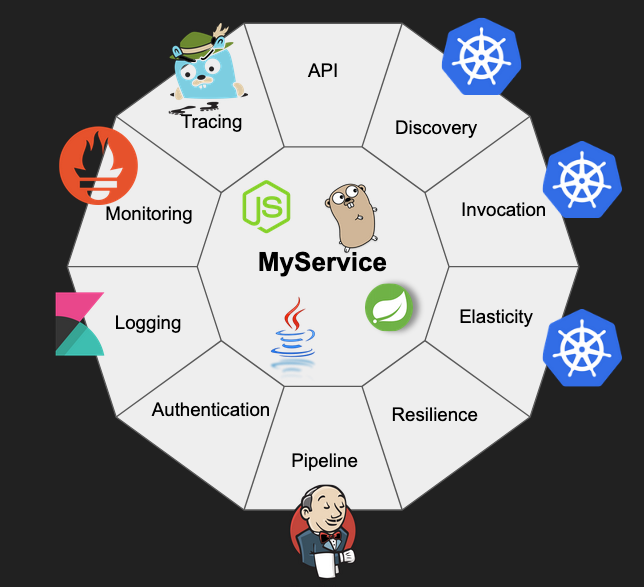
\includegraphics[width=0.5\linewidth]{Images/kube2.png}
        \label{fig:container}
    \end{figure}

    Créditos: Rafael Benevides
\end{frame}


\begin{frame}{Kubernetes}
    \begin{figure}
        \centering
        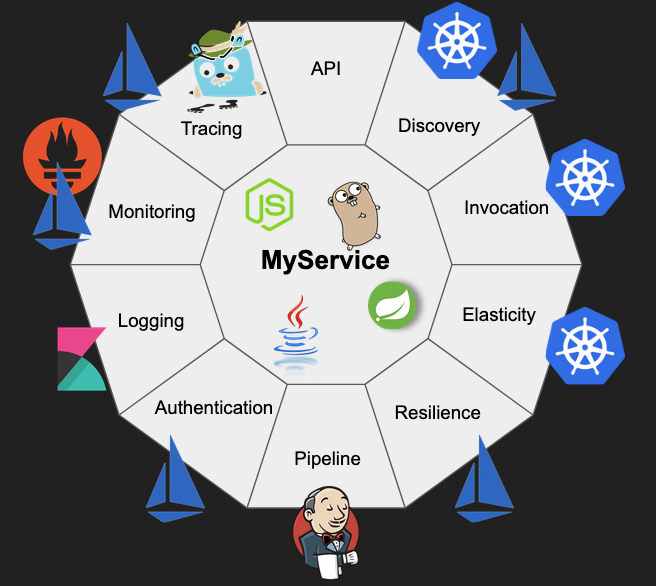
\includegraphics[width=0.5\linewidth]{Images/kube3.png}
        \label{fig:container}
    \end{figure}

    Créditos: Rafael Benevides
\end{frame}

\begin{frame}{Kubernetes}
    \begin{figure}
        \centering
        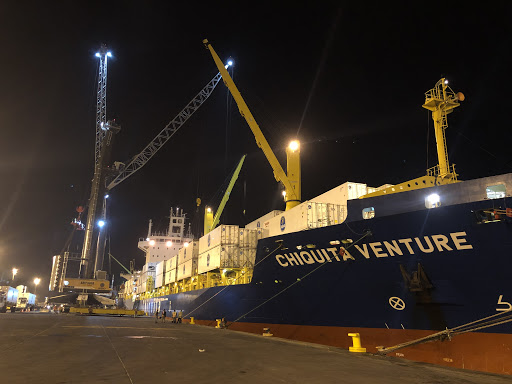
\includegraphics[width=0.8\linewidth]{Images/kubquetzal}
    \end{figure}
\end{frame}

{
    \usebackgroundtemplate{
\includegraphics[width=\paperwidth]{Images/separador}}
    \setbeamercolor{normal text}{fg=white}
    \setbeamercolor{frametitle}{fg=red}
    \usebeamercolor[fg]{normal text}
    \section{Conceptos generales}
}

\begin{frame}{Kubernetes}

    \begin{alertblock}{¿Que es un Kubernetes?}
        \begin{itemize}
            \item Orquestador
            \item Cluster de ejecución
        \end{itemize}
    \end{alertblock}

\end{frame}

\begin{frame}{Kubernetes}

    \begin{alertblock}{Cluster}
        \begin{itemize}
            \item Master plane (Control plane)
            \item Data plane (Node)
            \item Kubernetes DNS
        \end{itemize}
    \end{alertblock}

\end{frame}

\begin{frame}{Kubernetes}
    \begin{figure}
        \centering
        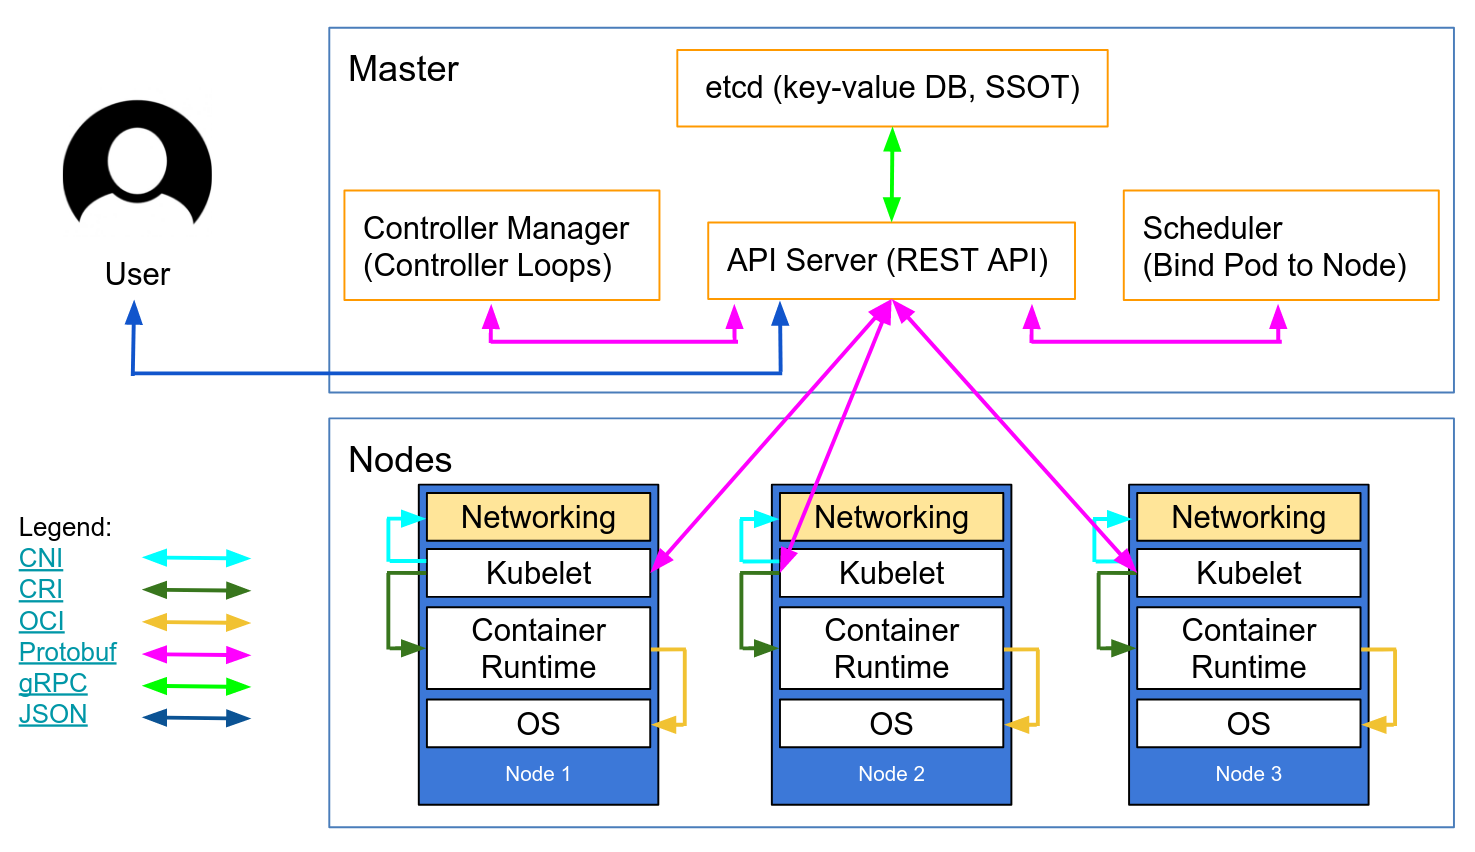
\includegraphics[width=0.7\linewidth]{Images/kuberarch.png}
    \end{figure}
Créditos: Nigel Poulton - The Kubernetes Book
\end{frame}

\begin{frame}{Kubernetes - Master}
    \begin{figure}
        \centering
        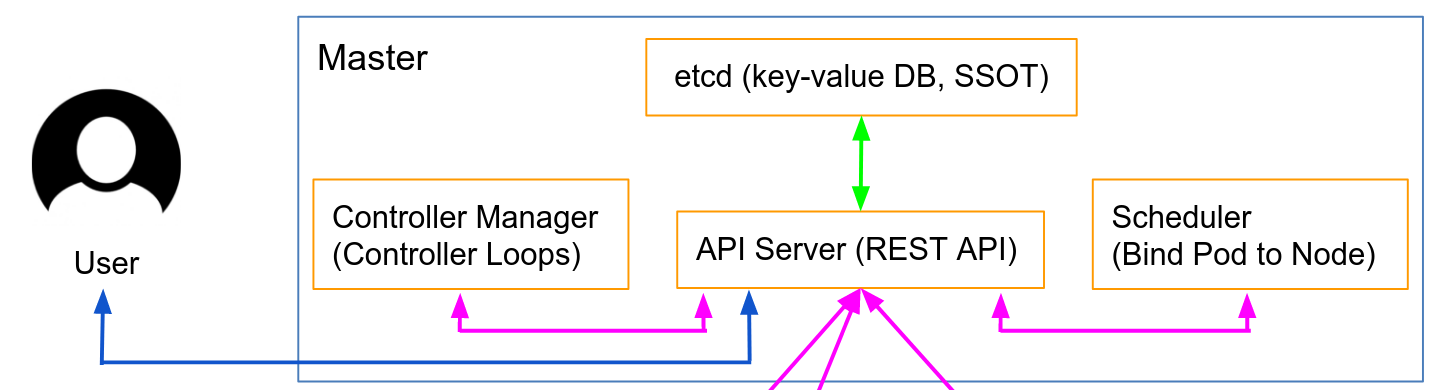
\includegraphics[width=0.8\linewidth]{Images/kuberarchmaster.png}
    \end{figure}
Créditos: Nigel Poulton - The Kubernetes Book
\end{frame}



\begin{frame}{Kubernetes - Master}

    \begin{exampleblock}{Elementos}
        \begin{enumerate}
            \item API server:
            \item Cluster store
            \item Controller manager
            \item Scheduler
            \item Cloud controller manager
        \end{enumerate}
    \end{exampleblock}

\end{frame}

\begin{frame}{Kubernetes - Node}
    \begin{figure}
        \centering
        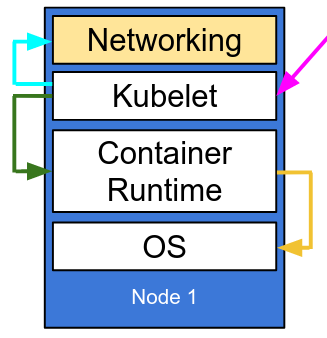
\includegraphics[width=0.3\linewidth]{Images/kuberarchnode.png}
    \end{figure}
Créditos: Nigel Poulton - The Kubernetes Book
\end{frame}



\begin{frame}{Kubernetes - Node}

    \begin{exampleblock}{Elementos}
        \begin{enumerate}
            \item Kubelet
            \item CRI
            \item Kube-Proxy
        \end{enumerate}
    \end{exampleblock}

\end{frame}

{
    \usebackgroundtemplate{
\includegraphics[width=\paperwidth]{Images/separador}}
    \setbeamercolor{normal text}{fg=white}
    \setbeamercolor{frametitle}{fg=red}
    \usebeamercolor[fg]{normal text}
    \section{Empaquetando aplicaciones}
}


\begin{frame}{Kubernetes - Empaquetado}

            \begin{exampleblock}{Proceso}
                \begin{itemize}
                    \item Aplicación debe estar en contenedor
                    \item Contenedor se declara en Pod
                    \item Pod se utiliza (opcionalmente) en Deployment
                \end{itemize}
            \end{exampleblock}

\end{frame}

\begin{frame}{Kubernetes - Empaquetado}
    \begin{figure}
        \centering
        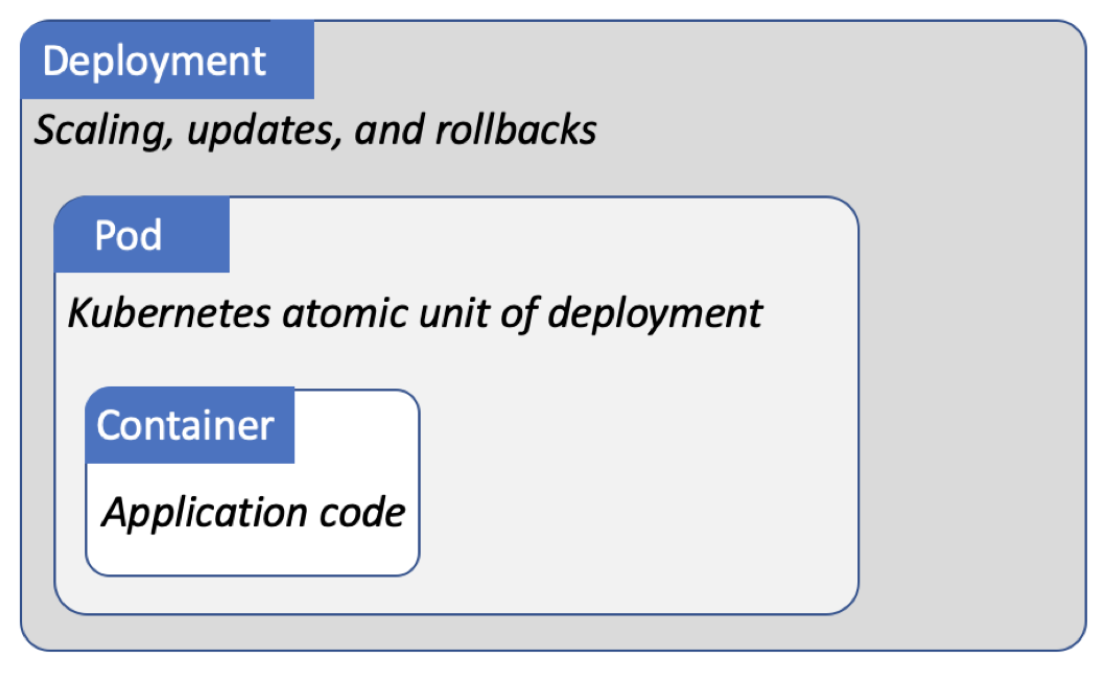
\includegraphics[width=0.7\linewidth]{Images/deploymentpodcontainer.png}
    \end{figure}
Créditos: Nigel Poulton - The Kubernetes Book
\end{frame}



\begin{frame}{Kubernetes - Empaquetado}

    \begin{exampleblock}{Secuencia de ejecución}
        \begin{itemize}
            \item Estado se encuentra en archivo manifest (YAML)
            \item Estado se envia (POST) hacia API server
            \item Kubernetes almacena el estado como \textit{desired}
            \item Kubernetes implementa el estado en el cluster
            \item Kubernetes reconcilia constantemente \textit{current state} con \textit{desired state}
        \end{itemize}
    \end{exampleblock}

\end{frame}




\begin{frame}{Kubernetes - Pod}

Pod of Whales

            \begin{alertblock}{¿Que es un pod?}
                \begin{itemize}
                    \item Uno o más  vinculados
                    \item IP Compartida
                    \item Caen todos o ninguno (ciclo de vida)
                    \item Storage compartido
                    \item Recursos compartidos
                \end{itemize}
            \end{alertblock}

\end{frame}

\begin{frame}{Kubernetes - Pod}

Casos de multiples containers

                \begin{itemize}
                    \item Service mesh
                    \item Helper container
                    \item Log scrapper
                \end{itemize}

\end{frame}


\begin{frame}{Kubernetes - Pod}
    \begin{figure}
        \centering
        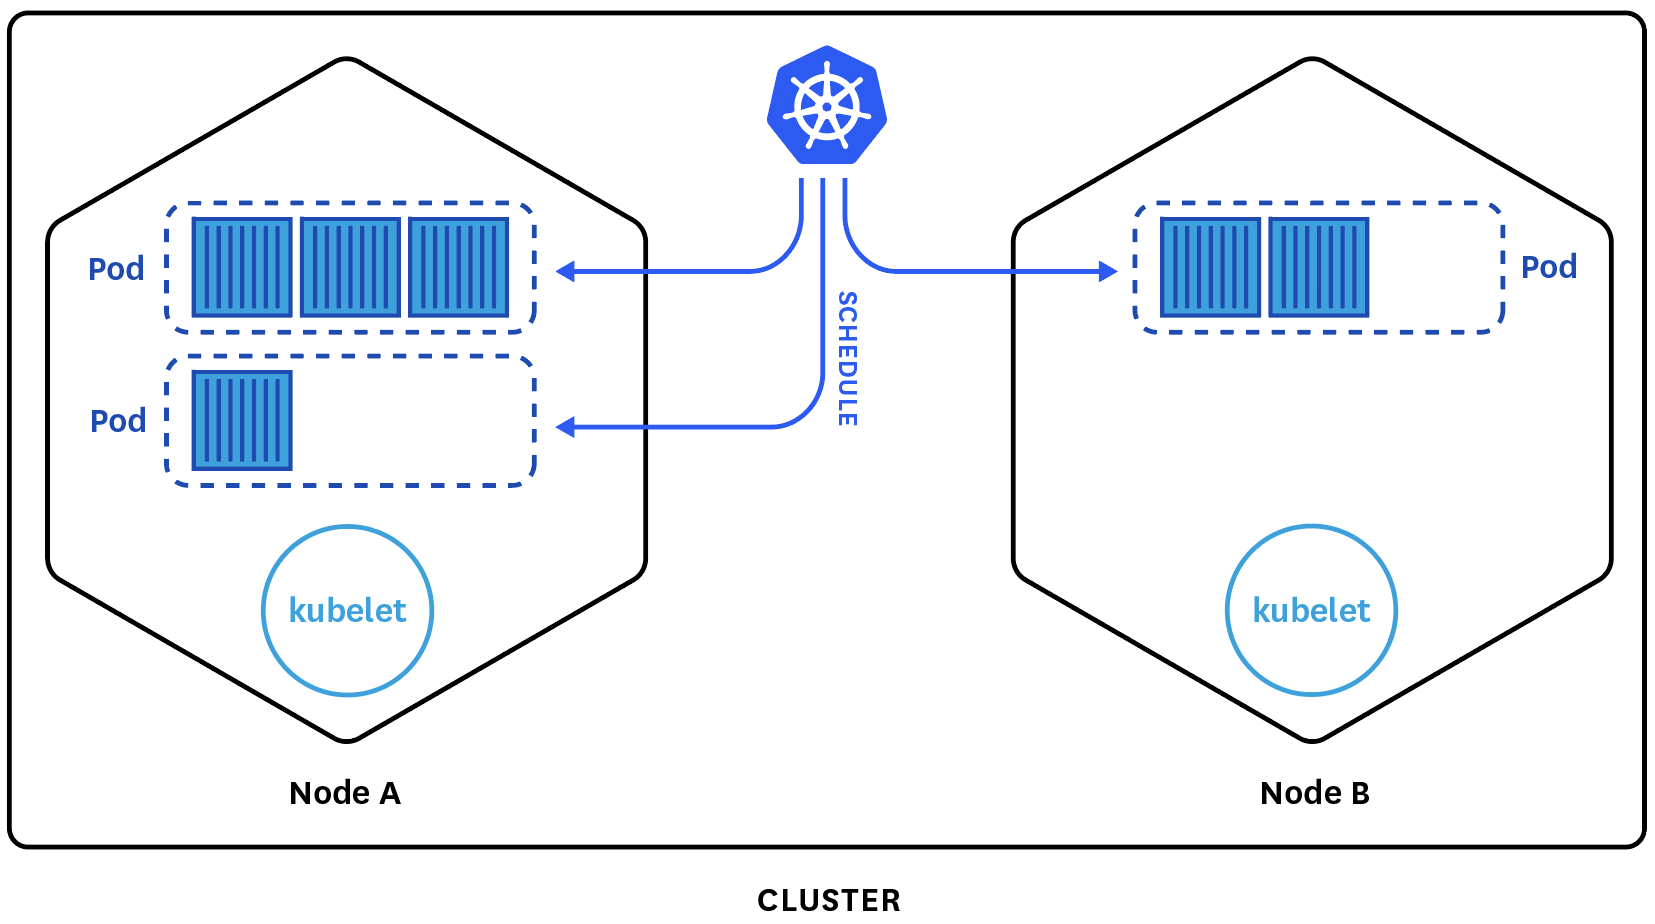
\includegraphics[width=0.7\linewidth]{Images/kubernetespods.png}
    \end{figure}
Créditos: Nigel Poulton - The Kubernetes Book
\end{frame}


\begin{frame}{Kubernetes - Pod}
    \begin{figure}
        \centering
        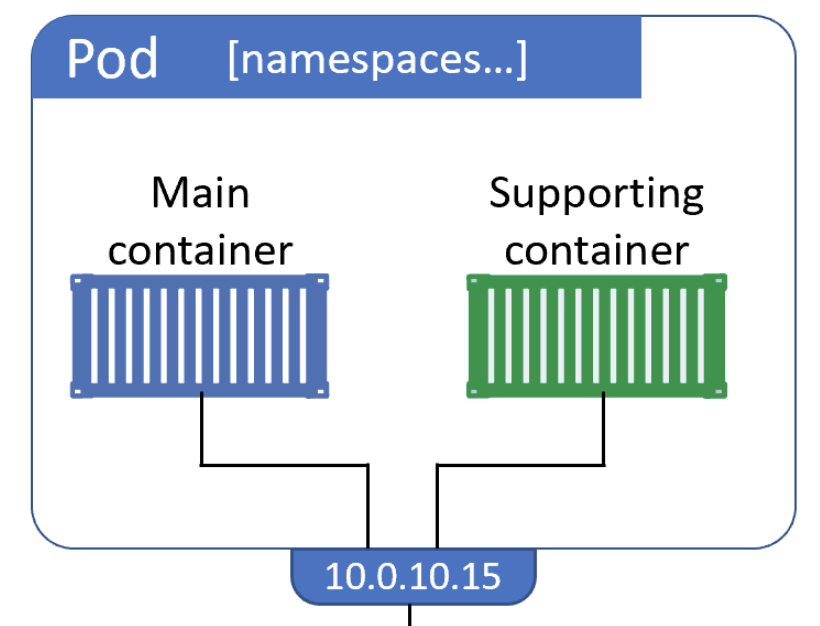
\includegraphics[width=0.55\linewidth]{Images/podanatomy.png}
    \end{figure}
Créditos: Nigel Poulton - The Kubernetes Book
\end{frame}

\begin{frame}{Kubernetes - Pod}

Kernel ring fenced

                \begin{itemize}
                    \item Red (Ip)
                    \item Kernel Namespace
                    \item IPC
                    \item Memory space
                    \item Volumes
                \end{itemize}

Desplegables con
\begin{itemize}
    \item Deployments
    \item Daemon Sets
    \item Stateful Sets
\end{itemize}

\end{frame}



\begin{frame}{Kubernetes - Deployment}

    \begin{alertblock}{¿Que es un deployment?}
        Descriptor que mantiene el número de PODs/replicas en ejecución. Describe un estado
    \end{alertblock}


\end{frame}


\begin{frame}{Kubernetes - Servicios}

    \begin{alertblock}{¿Que es un servicio?}
        Agrupación de PODs de una misma naturaleza, -e.g. una IP estable virtual y un nombre de DNS para replicas de un servicio-
    \end{alertblock}


\end{frame}

\begin{frame}{Kubernetes - Servicios}
    \begin{figure}
        \centering
        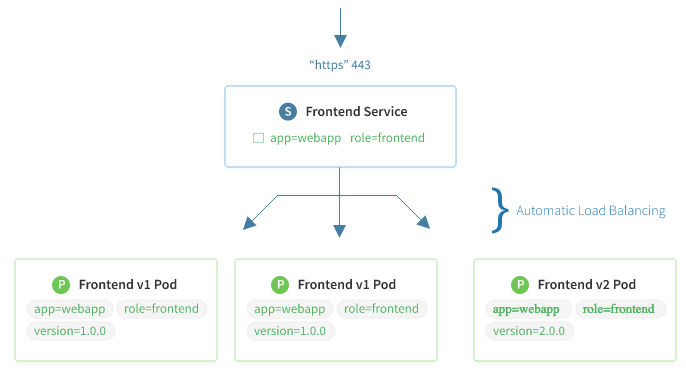
\includegraphics[width=0.65\linewidth]{Images/kubernetesservice.png}
    \end{figure}
\end{frame}




{
    \usebackgroundtemplate{
\includegraphics[width=\paperwidth]{Images/separador}}
    \setbeamercolor{normal text}{fg=white}
    \setbeamercolor{frametitle}{fg=red}
    \usebeamercolor[fg]{normal text}
    \section{Probando kubernetes}
}

\begin{frame}{Kubernetes - Pruebas}

    \begin{itemize}
        \item \textbf{PWK}
        \item \textbf{Docker Desktop}
        \item Minikube
    \end{itemize}

\end{frame}


\begin{frame}{Kubernetes - Servicios}

    \begin{itemize}
        \item Red estable
        \item Punto de abstracción
        \item Balanceo TPC/UDP
        \item Label = Etiqueta para decidir si entra en balanceo
    \end{itemize}

    Tipos
    \begin{itemize}
            \item Cluster IP
            \item NodePort
            \item LoadBalancer
            \item Externa name
        \end{itemize}
\end{frame}

\begin{frame}{Kubernetes - Servicios}
    \begin{figure}
        \centering
        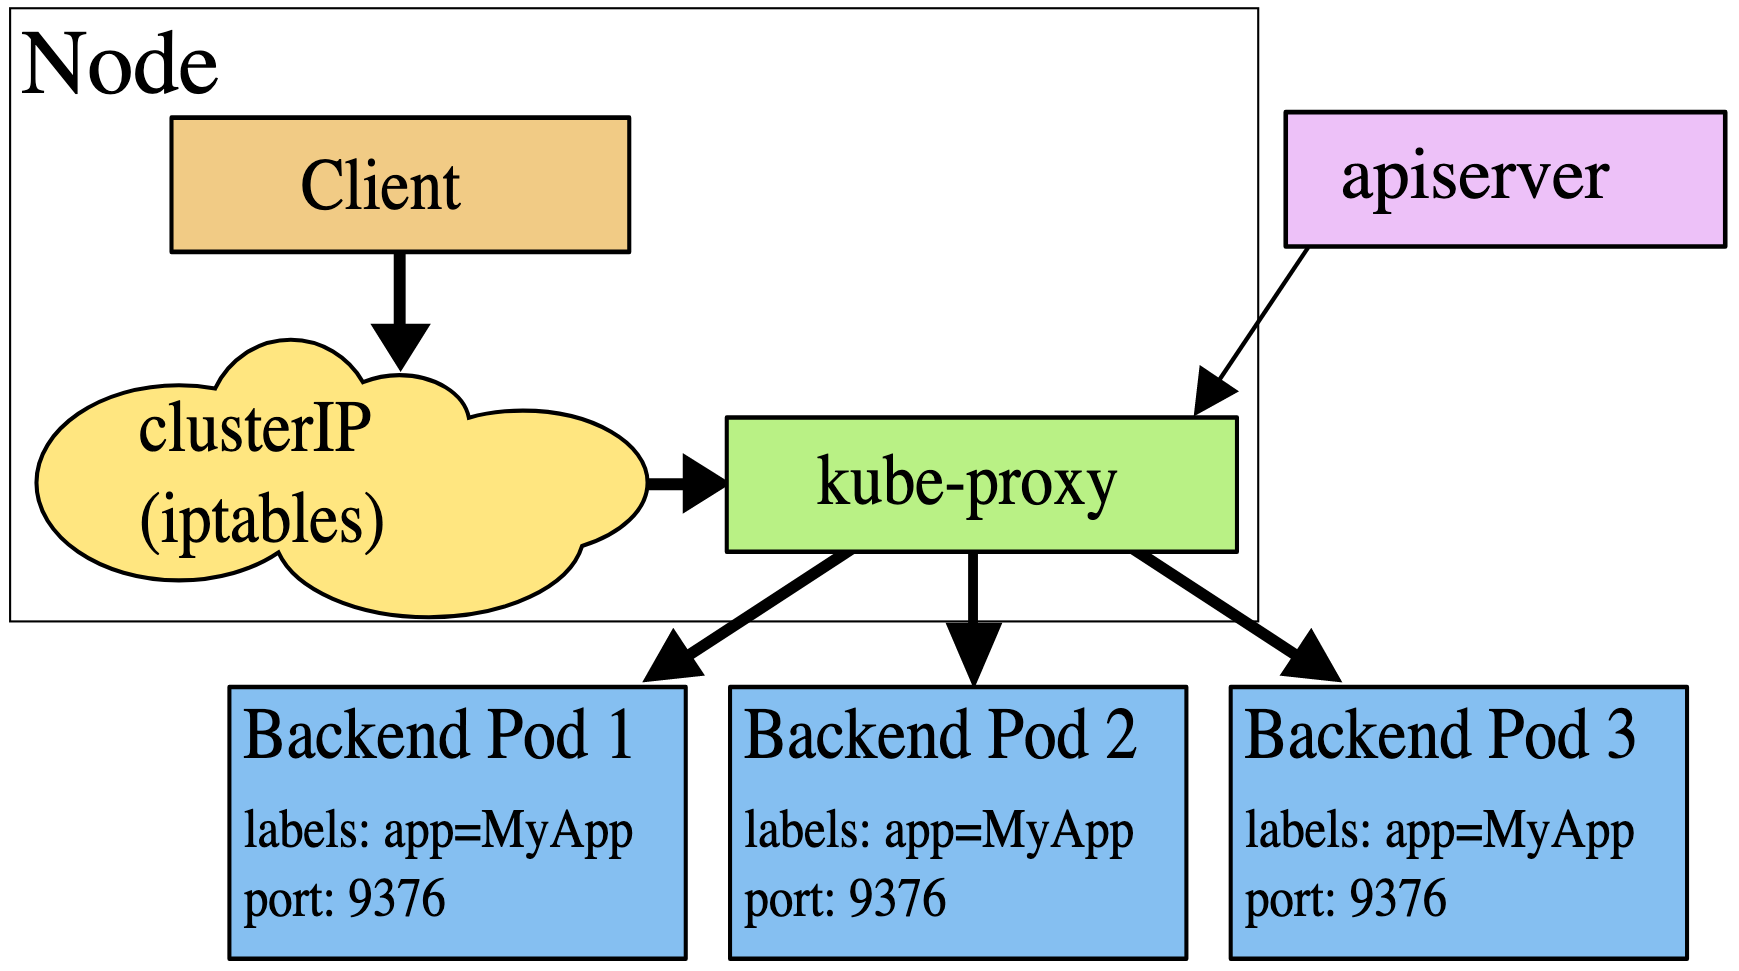
\includegraphics[width=0.65\linewidth]{Images/kubeservice1.png}
    \end{figure}
Créditos: Nigel Poulton - The Kubernetes Book
\end{frame}


\begin{frame}{Kubernetes - Servicios}
    \begin{figure}
        \centering
        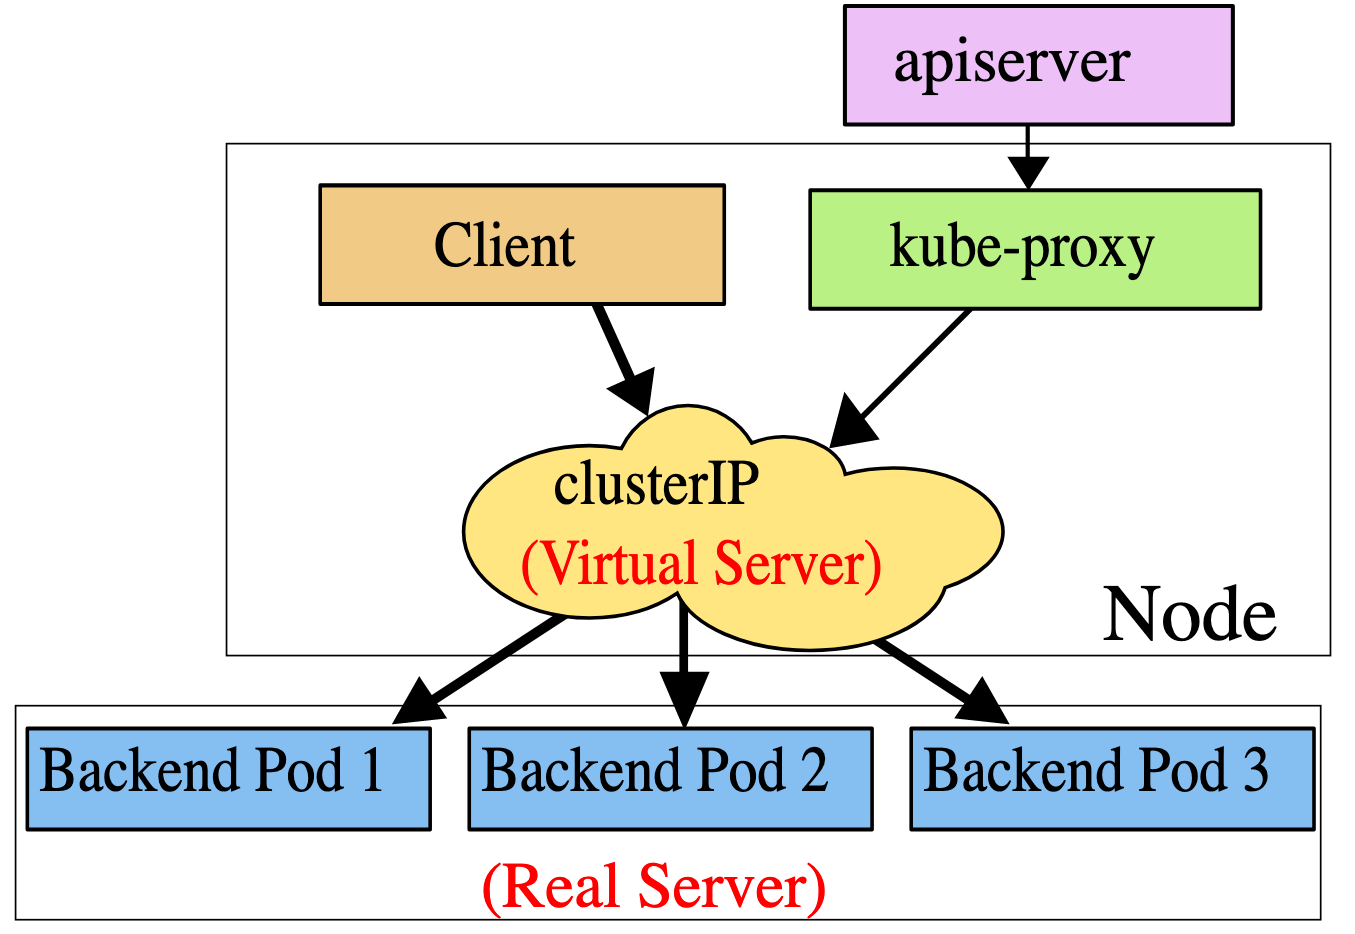
\includegraphics[width=0.55\linewidth]{Images/kubeservice2.png}
    \end{figure}
Créditos: Nigel Poulton - The Kubernetes Book
\end{frame}



\begin{frame}{Kubernetes - Elementos canonicos}

    \begin{itemize}
        \item API
        \item Kind
        \item Metadata
 \item Spec
    \end{itemize}

\end{frame}

\begin{frame}{Víctor Orozco}
\begin{columns}[T] % contents are top vertically aligned

	\begin{column}[T]{4cm} % alternative top-align that's better for graphics
		\begin{figure}
			\centering
			
\includegraphics[width=\linewidth]{Images/logos}
		\end{figure}
	\end{column}
	\begin{column}[T]{6cm} % each column can also be its own environment
		\begin{itemize}
			\item vorozco@nabenik.com
			\item \href{https://twitter.com/tuxtor}{@tuxtor}
			\item \href{http://vorozco.com}{http://vorozco.com}
			\item \href{http://tuxtor.shekalug.org}{http://tuxtor.shekalug.org}
		\end{itemize}
		\begin{center}
			
\includegraphics[width=0.1\linewidth]{Images/cclogo}
			\\
			This work is licensed under Creative Commons Attribution-NonCommercial-ShareAlike 3.0 Guatemala (CC BY-NC-SA 3.0 GT).
		\end{center}
	\end{column}
\end{columns}
\end{frame}

{
    \usebackgroundtemplate{
\includegraphics[width=\paperwidth]{Images/final}}
    \begin{frame}
    \end{frame}
}


\end{document}

